\documentclass[sigconf]{acmart}



% \setcopyright{acmlicensed}
% \copyrightyear{2024}
% \acmYear{2024}
% \acmDOI{XXXXXXX.XXXXXXX}

\acmConference{Geometry Data Analysis}{December 2024}{Paris, France}

\acmISBN{978-1-4503-XXXX-X/18/06}
\begin{document}
%%
%% The "title" command has an optional parameter,
%% allowing the author to define a "short title" to be used in page headers.
\title{Analysis over the Vector Heat Method}

%%
%% The "author" command and its associated commands are used to define
%% the authors and their affiliations.
%% Of note is the shared affiliation of the first two authors, and the
%% "authornote" and "authornotemark" commands
%% used to denote shared contribution to the research.
\author{Ícel Viñals Pierigé}
\affiliation{%
  \institution{\'Ecole nationale des Ponts et Chaussées}
  \city{Champs-sur-Marne}
  \country{France}}
\email{icel.vinals-pierige@enpc.fr}

\author{Cécile Liu}
\affiliation{%
  \institution{\'Ecole nationale des Ponts et Chaussées}
  \city{Champs-sur-Marne}
  \country{France}}
\email{cecile.liu@enpc.fr}

\author{Nicolas Sereyjol-Garros}
\affiliation{%
  \institution{\'Ecole nationale des Ponts et Chaussées}
  \city{Champs-sur-Marne}
  \country{France}}
\email{nicolas.sereyjol-garros@enpc.fr}


\begin{abstract}
  A clear and well-documented \LaTeX\ document is presented as an
  article formatted for publication by ACM in a conference proceedings
  or journal publication. Based on the ``acmart'' document class, this
  article presents and explains many of the common variations, as well
  as many of the formatting elements an author may use in the
  preparation of the documentation of their work.
\end{abstract}

%%
%% The code below is generated by the tool at http://dl.acm.org/ccs.cfm.
%% Please copy and paste the code instead of the example below.
%%
\begin{CCSXML}
<ccs2012>
   <concept>
       <concept_id>10010147.10010371.10010396.10010402</concept_id>
       <concept_desc>Computing methodologies~Shape analysis</concept_desc>
       <concept_significance>500</concept_significance>
       </concept>
   <concept>
       <concept_id>10002950.10003714.10003715.10003750</concept_id>
       <concept_desc>Mathematics of computing~Discretization</concept_desc>
       <concept_significance>500</concept_significance>
       </concept>
   <concept>
       <concept_id>10002950.10003714.10003727.10003729</concept_id>
       <concept_desc>Mathematics of computing~Partial differential equations</concept_desc>
       <concept_significance>500</concept_significance>
       </concept>
 </ccs2012>
\end{CCSXML}

\ccsdesc[500]{Computing methodologies~Shape analysis}
\ccsdesc[500]{Mathematics of computing~Discretization}
\ccsdesc[500]{Mathematics of computing~Partial differential equations}

%%
%% Keywords. The author(s) should pick words that accurately describe
%% the work being presented. Separate the keywords with commas.
\keywords{discrete differential geometry, parallel
transport, velocity extrapolation, logarithmic map, exponential map, Karcher
mean, geometric median}

\begin{teaserfigure}
  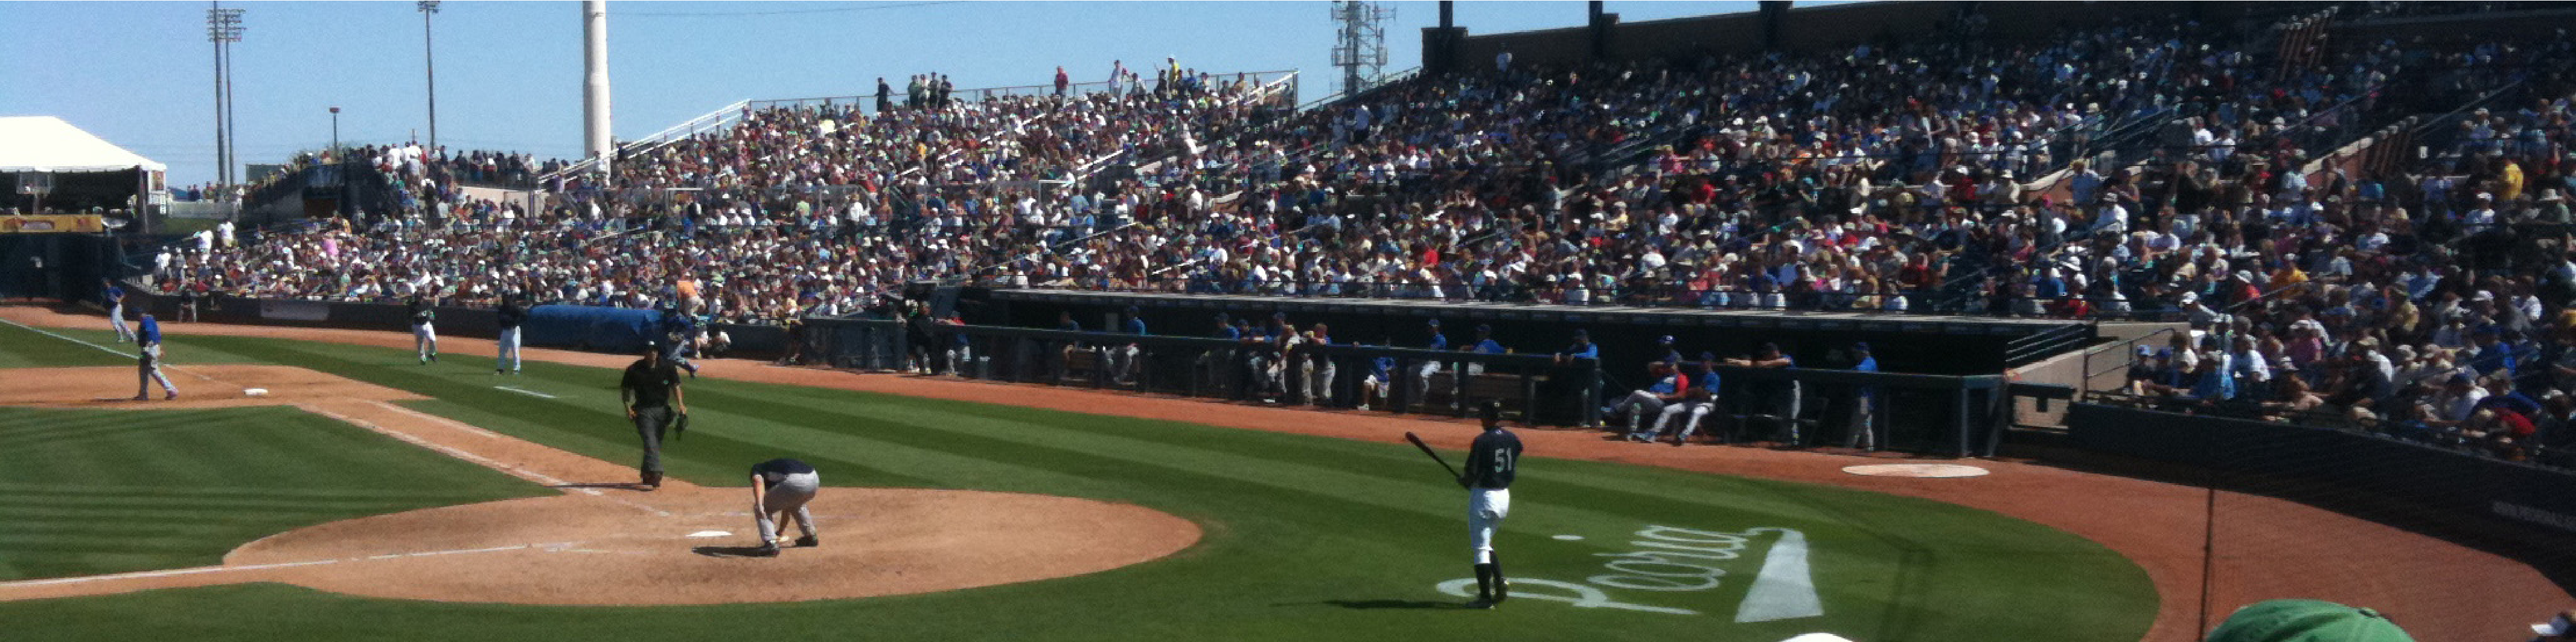
\includegraphics[width=\textwidth]{sampleteaser}
  \caption{Seattle Mariners at Spring Training, 2010.}
  \Description{Enjoying the baseball game from the third-base
  seats. Ichiro Suzuki preparing to bat.}
  \label{fig:teaser}
\end{teaserfigure}

\received{20 February 2007}
\received[revised]{12 March 2009}
\received[accepted]{5 June 2009}

%%
%% This command processes the author and affiliation and title
%% information and builds the first part of the formatted document.
\maketitle

\section{Introduction}
\section{BRAIN STORM:}
\begin{itemize}
  \item Test robustness with a custom mesh + noise (similar to what they did) and mesh+crossed triangles (shortcuts should break the results?)
  \item Test different step sizes (t's) verify that 1 seems to be the best
  \item Compare results numerically with 'perfect' algorithm from https://hhoppe.com/geodesics.pdf
  \item Find how to test with different data types (point clouds, triang meshes, poly meshes) and compare results (if possible in software without too much rewriting?)
  \item Try results on bad vs good triangulated meshes (to check if Delaunay works fine)
  \item Think about new possible applications? Videogames/3d animation?? 
  \item Check 2020 method to compute geodesics only by flipping triangles. One advantage seems to be that it works to find not only global shortest paths, but also local ones (if two points are next to each other, it can find the shortest path in the opposite direction by turning around)  https://dl.acm.org/doi/10.1145/3414685.3417839
  \item Test speed against fast marching method for scalar heat method
  \item Check behaviour at Cut locus and comment it
\end{itemize}
\section{Travail à faire:}
\begin{itemize}
  \item Test different step sizes (t's) verify that 1 seems to be the best ()
  \item Check behaviour at Cut locus and comment it
  \item Test robustness with a custom mesh + noise (similar to what they did) and mesh+crossed triangles (shortcuts should break the results?)(Icel)
  \item Compare results numerically with 'perfect' algorithm from https://hhoppe.com/geodesics.pdf
  \item Find how to test with different data types (point clouds, triang meshes, poly meshes) and compare results (if possible in software without too much rewriting?)
  \item Try results on bad vs good triangulated meshes (to check if Delaunay works fine)
  \item Think about new possible applications? Videogames/3d animation?? 
  \item Check 2020 method to compute geodesics only by flipping triangles. One advantage seems to be that it works to find not only global shortest paths, but also local ones (if two points are next to each other, it can find the shortest path in the opposite direction by turning around)  https://dl.acm.org/doi/10.1145/3414685.3417839
  \item Test speed against fast marching method for scalar heat method
  \item Test times for prepocessing time
\end{itemize}

\begin{itemize}
  \item Test application: put a texture on a moving 3d model to check coherency
  \item Look for applications for the Karcher mean
\end{itemize}

\section{Context}



\section{Solution}
\section{Limits}






\bibliographystyle{ACM-Reference-Format}
\bibliography{sample-base}

\end{document}

\endinput
%%
%% End of file `sample-sigconf-authordraft.tex'.
